\documentclass{IEEEtran}
\usepackage[utf8]{inputenc}
\usepackage[alsoload=synchem,load=named]{siunitx}
\usepackage{graphicx}
\usepackage{breqn}
\usepackage{booktabs, tabularx}
\usepackage{hyperref}
\usepackage{listings}
\usepackage[citestyle=ieee,sorting=none,bibencoding=utf8,backend=biber]{biblatex}

\graphicspath{{images/}}
\bibliography{bibliography}

\author{J.R. Powers-Luhn}
\title{Homework 2: Data Statistics}
\date{September 11th, 2018}

\DeclareSIUnit\year{yr}
\DeclareSIUnit\inch{in}

\begin{document}
\maketitle

\section{Abstract}
Prior to generating \textit{post hoc} models from data it is necessary to examine the data to validate any assumptions made in collecting it. That examination should include explicitly stated assumptions as well as attempts to validate those assumptions prior to drawing conclusions about the data. Generating models from biased data can obviously result in biased models, but those biases may be more subtle in the model than in the data that produced it. In order to demonstrate the form that such an examination might take, statistical summary calculations were performed on data collected for a 1985 body weight study. It was determined that the sampled data did not conform to expected (Gaussian) distributions, and that at least one significant outlier was present in a parameter used to calculate lean body mass in the 1985 paper. An examination was made of the cross-correlations between the measured data and the body fat percentage predictions, revealing that abdominal circumference may be a good predictor of body fat percentage (correlation value of $0.81$). 

\section{Introduction}
Understanding the distribution of a signal with a random component is a necessary first step in analyzing or modeling that signal. In order to recover the true nature of a physical phenomena, we measure the value of the signal plus some random noise, $M = S + N$. Misunderstanding the noise results in misunderstanding the recovered signal, which may lead to incorrect conclusions about the data. If the noise is underestimated then this could lead to a true hypothesis being rejected. Similarly, mischaracterizing the distribution from which the noise is generated could result in a systematic bias in models. 

\subsection{Gaussian Distribution}
A common physical model for a single sampled quantity is a mean value plus some variation drawn from a Gaussian distribution, as in equation \ref{eq:gauss}.

\begin{equation}
	G(x | \mu, \sigma) = \frac{1}{\sqrt{2 \pi \sigma^2}} \mathrm{e}^{-\frac{(x-\mu)^2}{2 \sigma^2}}
	\label{eq:gauss}
\end{equation}

This assumption, however, is not always valid. In order to test this, we can compare the properties of the measured distribution to the hypothetical distribution by measuring the mathematical properties called \textit{moments}. The $n$th moment of a distribution is described by equation \ref{eq:moment}.

\begin{equation}
	\mu_n = \int_{\infty}^{\infty} (x - c)^n f(x) dx
	\label{eq:moment}
\end{equation}

The moments of a set of samples (plus some other characteristics: the median, trimmed mean, and standard deviation) are characteristic of a distribution. In order to illustrate this, statistical properties were calculated for a real-life data set made of sampled data \cite{Penrose1985}. This data set consists of 252 samples each of fourteen quantities:

\begin{itemize}
	\item Age (\si{\year})
	\item Weight (lbs)
	\item Height (inches)
	\item Adiposity index (\si{\kilo\gram\per\meter^2})
	\item Neck circumference (\si{\centi\meter})
	\item Chest circumference (\si{\centi\meter})
	\item Ab circumference (\si{\centi\meter})
	\item Hip circumference (\si{\centi\meter})
	\item Thigh circumference (\si{\centi\meter})
	\item Knee circumference (\si{\centi\meter})
	\item Ankle circumference (\si{\centi\meter})
	\item Extended bicep circumference (\si{\centi\meter})
	\item Forearm circumference (\si{\centi\meter})
	\item Wrist circumference (\si{\centi\meter})
\end{itemize}

\num{143} of these measured values were used to derive the lean body weight equation \ref{eq:brozek}, with abdominal ($Ab$) and wrist ($Wr$) circumferences measured in \si{\centi\meter}, weight ($Wt$) measured in \si{\kilo\gram}, and height ($Hgt$) measured in \si{\meter}. This was then validated with \num{109} additional measurements. From this it was expected that lean body weight would be strongly positively correlated with weight and height, weakly positively correlated with wrist circumference, and somewhat negatively correlated with abdominal circumference. Because of the nonlinear correlation between age and lean body weight, it was expected that the correlation between these two values would be low. Additionally it was expected that percent body fat would inversely correlate with lean body weight.

\begin{dmath}
	LBW = 17.298 + 0.89946 (Wt) - 0.2783 (Age) + 0.002617 (Age^2) + 17.819 (Hgt) - 0.6798 (Ab - Wr)
	\label{eq:brozek}
\end{dmath}

Prior to examination, it was predicted that age would appear to conform to a nearly uniform distribution (possibly with a tail on the high end of the distribution) while all other sampled variable would appear to be Gaussian. 

\section{Results}

\subsection{Summary Statistics}

In order to determine the distribution of the sampled input variables, summary statistics were calculated for each variable. The results of these calculations are reported in table \ref{tab:summary_statistics}. 

\begin{table*}
\begin{tabular}{llrrrrrrrrr}
\toprule
{} &                     Parameter &     Max &    Min &        Mean &  Median &  20\% Trimmed Mean &  Standard Deviation &    Variance &  Skewness &   Kurtosis \\
\midrule
0  &                           Age &   81.00 &   22.0 &   44.88 &   43.00 &         44.44 &           12.58 &  158.18 &  0.28 &  -0.43 \\
1  &                        Weight &  363.15 &  118.5 &  178.92 &  176.50 &        176.55 &           29.33 &  860.30 &  1.20 &   5.14 \\
2  &                        Height &   77.75 &   29.5 &   70.15 &   70.00 &         70.25 &            3.66 &   13.36 & -5.35 &  58.34 \\
3  &               Adiposity Index &   48.90 &   18.1 &   25.44 &   25.05 &         25.056 &            3.64 &   13.26 &  1.55 &   6.56 \\
4  &            Neck circumference &   51.20 &   31.1 &   37.99 &   38.00 &         37.93 &            2.43 &    5.88 &  0.55 &   2.64 \\
5  &           Chest circumference &  136.20 &   79.3 &  100.82 &   99.65 &        100.13 &            8.41 &   70.79 &  0.68 &   0.94 \\
6  &         Abdomen circumference &  148.10 &   69.4 &   92.56 &   90.95 &         91.81 &           10.76 &  115.81 &  0.83 &   2.18 \\
7  &             Hip circumference &  147.70 &   85.0 &   99.90 &   99.30 &         99.33 &            7.15 &   51.12 &  1.49 &   7.30 \\
8  &           Thigh circumference &   87.30 &   47.2 &   59.40 &   59.00 &         59.13 &            5.24 &   27.45 &  0.82 &   2.59 \\
9  &            Knee circumference &   49.10 &   33.0 &   38.59 &   38.50 &         38.49 &            2.41 &    5.79 &  0.51 &   1.02 \\
10 &           Ankle circumference &   33.90 &   19.1 &   23.10 &   22.80 &         22.91 &            1.69 &    2.86 &  2.24 &  11.68 \\
11 &  Extended bicep circumference &   45.00 &   24.8 &   32.27 &   32.05 &         32.16 &            3.02 &    9.09 &  0.28 &   0.46 \\
12 &         Forearm circumference &   34.90 &   21.0 &   28.66 &   28.70 &         28.70 &            2.02 &    4.07 & -0.22 &   0.82 \\
13 &           Wrist circumference &   21.40 &   15.8 &   18.23 &   18.30 &         18.22 &            0.93 &    0.87 &  0.28 &   0.36 \\
14 &                  \% Bodyweight &   45.10 &    0.0 &   18.94 &   19.00 &         18.86 &            7.74 &   59.84 &  0.14 &  -0.32 \\
\bottomrule
\end{tabular}

\caption{Table of summary statistics for data recorded in \cite{Penrose1985}\label{tab:summary_statistics}}
\end{table*}

These statistics revealed that the distribution of the input variables was neither uniform nor Gaussian. Only three measured variables (neck circumference, abdomen circumference, and thigh circumference) had kurtosis values within $\pm1$ of \num{3}. Height had a kurtosis value of \num{58.35}, likely due to the presence of a single outlier $11.1\sigma$ below the mean value of \SI{70.15}{\inch}. In spite of the median and 20\% trimmed mean being ``robust to outliers'' \cite{Coble2018}, in general, the mean, median, and trimmed mean were close to each other (within \num{0.2} standard deviations of the sample), as shown in figure \ref{fig:robust}. 

\begin{centering}
\begin{figure}
\centering
\begin{center}
	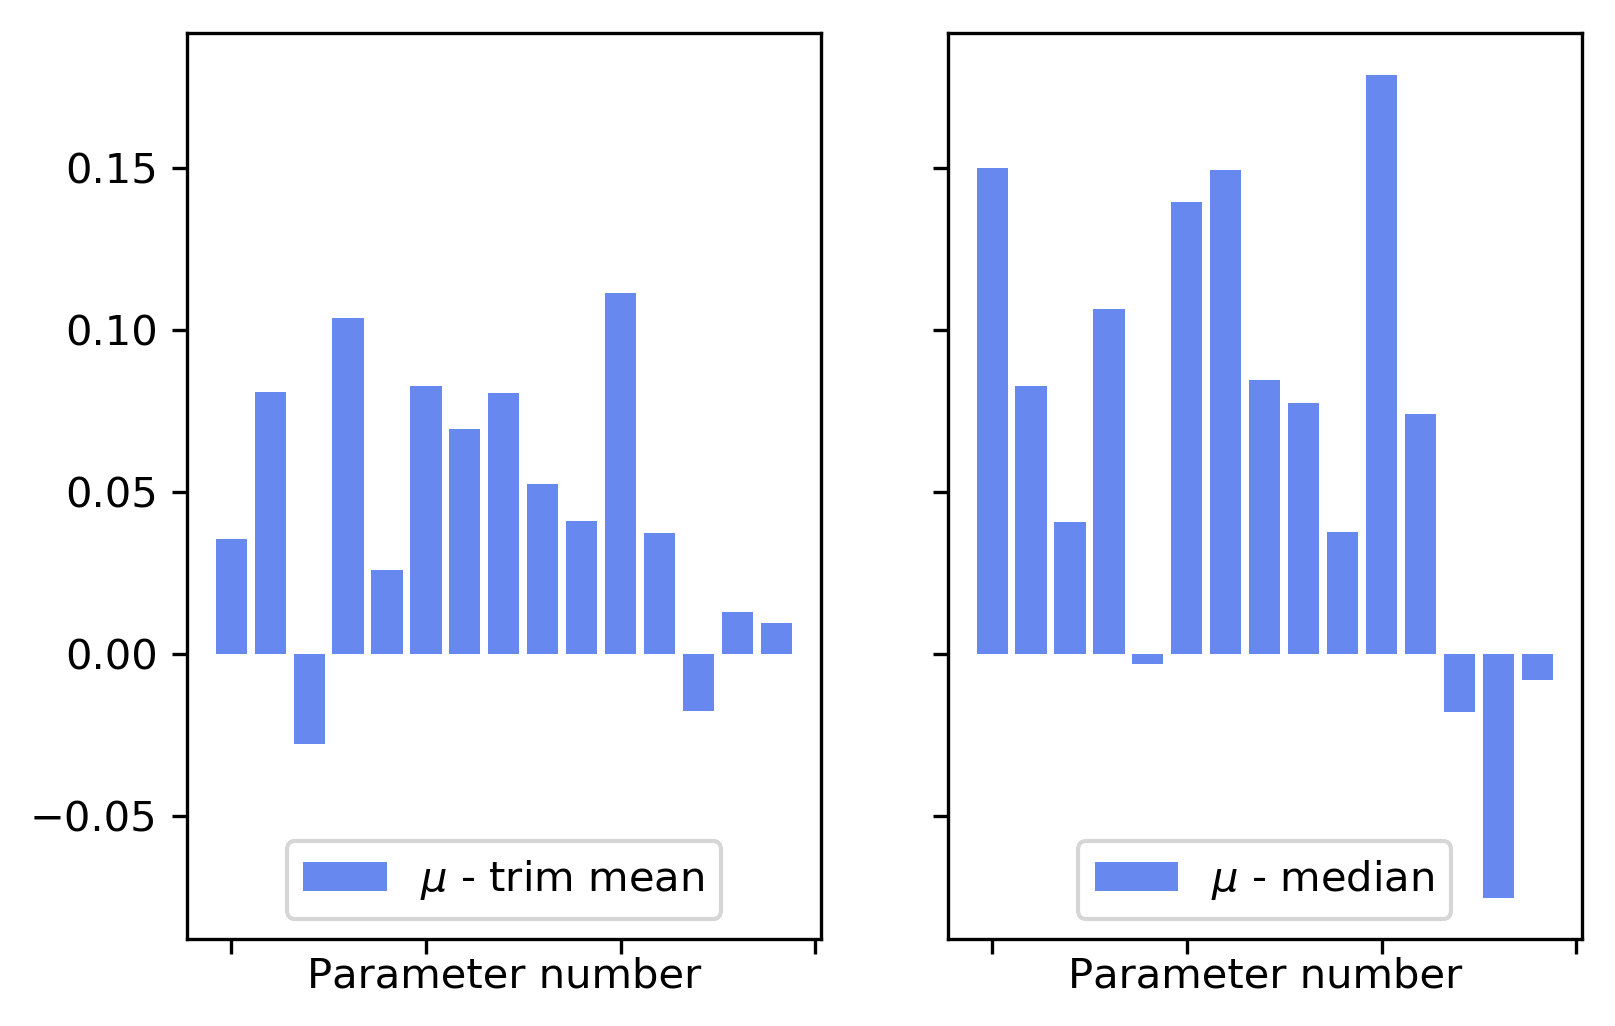
\includegraphics[width=0.5\textwidth]{robust_statistics}
	\caption{Separation between the mean and trimmed mean (left) and median (right), in units of standard deviation from the sampled data set. Height, the parameter with the furthest outlier, is represented by the third bar from the left. In spite of having the furthest outlier, it is in the smaller half of differences between the mean and either the trimmed mean or median.\label{fig:robust}}
\end{center}
\end{figure}
\end{centering}

In order to quickly process these distribution relative to the assumed Gaussian, histograms of the each distribution were plotted on the same axes as a Gaussian probability distribution function scaled to the number of observations in the data set (figure \ref{fig:gaussian_comparison}). Vertical lines were drawn to identify the mean of each variable. This serves to illustrate the deviation of each sampled variable from a Gaussian distribution.

\begin{centering}
\begin{figure}
\centering
\begin{center}
	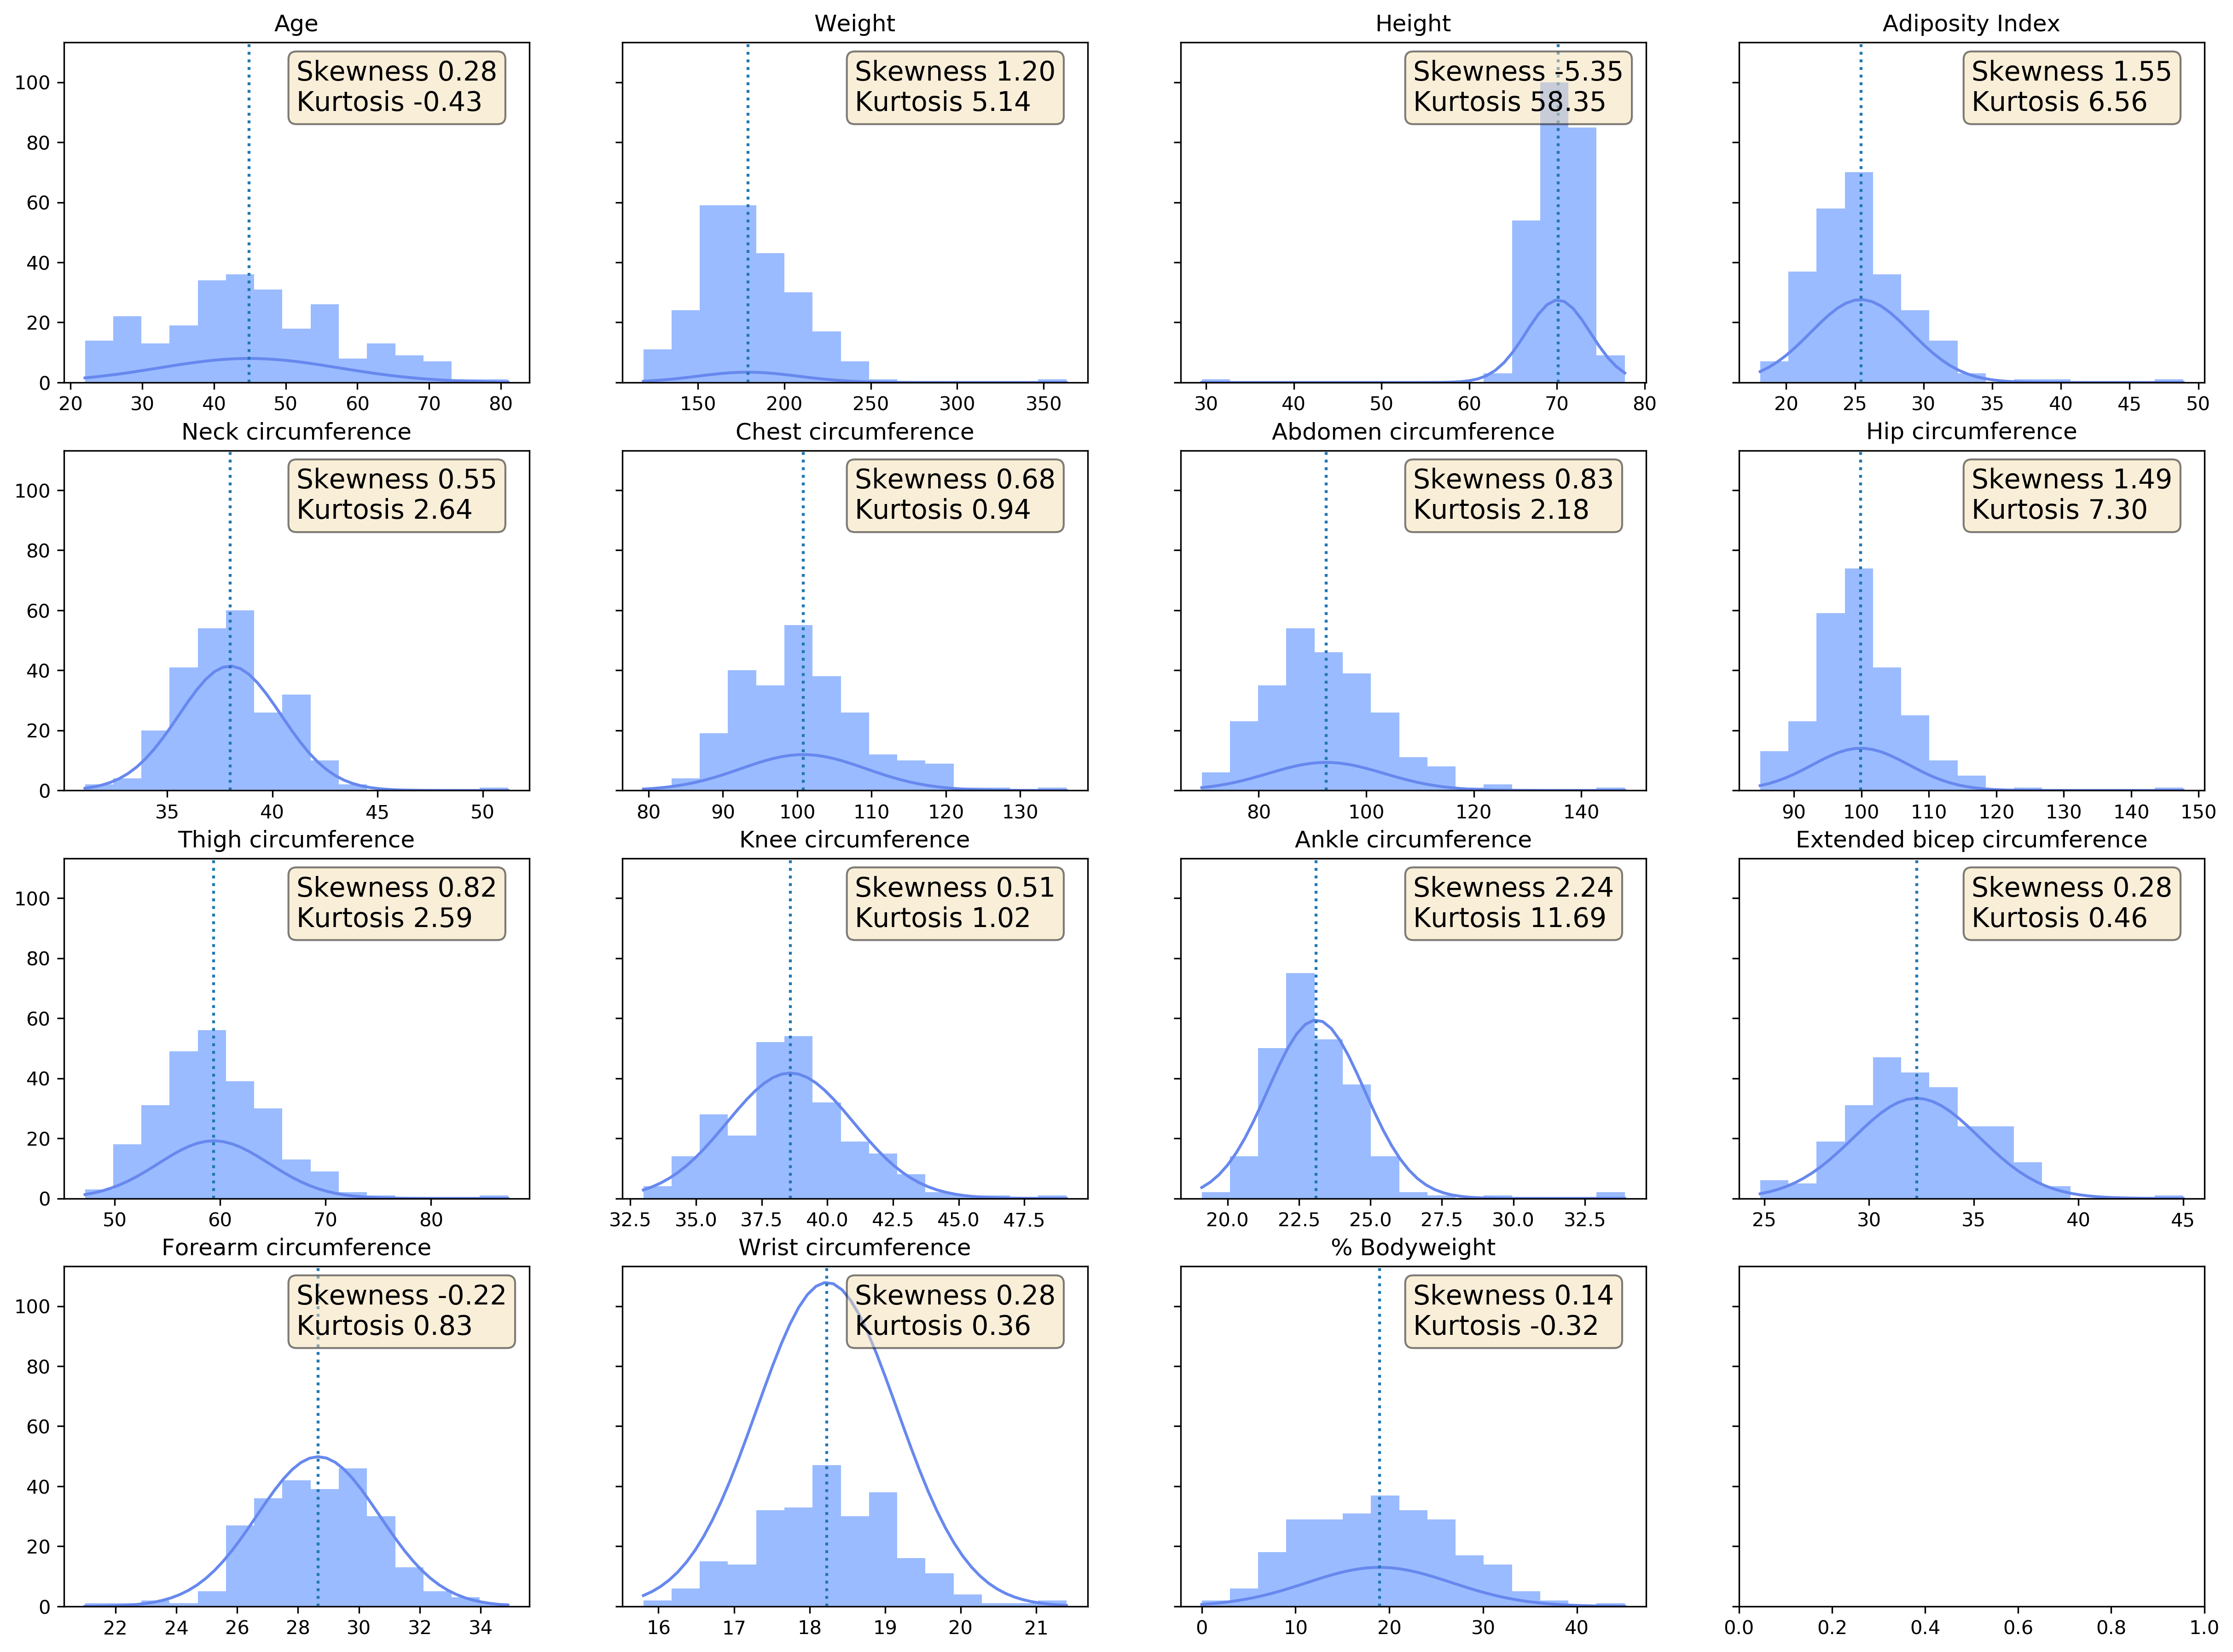
\includegraphics[width=0.5\textwidth]{histogram_array}
	\caption{Comparison of measured data to Gaussian distribution. The histogram for each measured parameter is overlayed with a Gaussian probability distribution function with the same mean and standard deviation. Higher-order moments (skewness and kurtosis) are listed in the insets.\label{fig:gaussian_comparison}}
\end{center}
\end{figure}
\end{centering}

This does not necessarily indicate that the underlying population does not follow a Gaussian distribution. To illustrate this, figure \ref{fig:sample_size} shows four normalized histograms drawn from the same population. The sample size for each histogram is shown above the plot. 

\begin{centering}
\begin{figure}
\centering
\begin{center}
	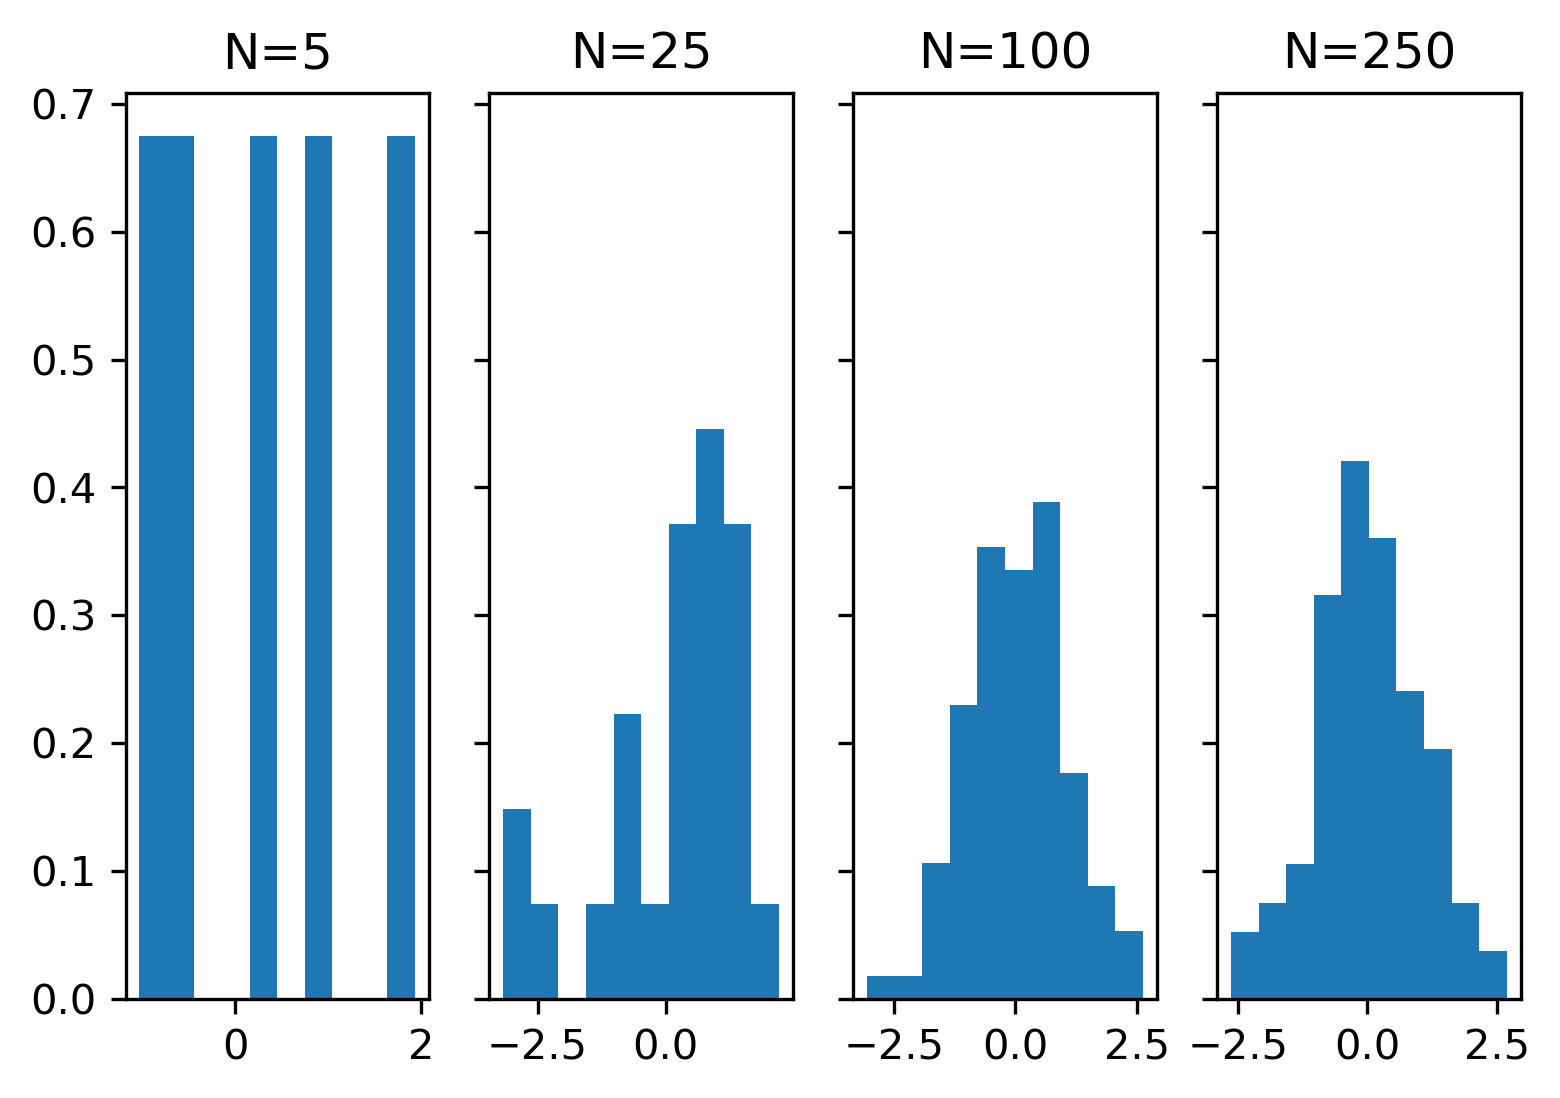
\includegraphics[width=0.5\textwidth]{sample_size}
	\caption{Four normalized sample distributions drawn from the same population. Small sample sizes result in difficulty identifying the distribution of the underlying population, and even large sample sizes may still result in a sample with different moments than the population that produced them.\label{fig:sample_size}}
\end{center}
\end{figure}
\end{centering}

\subsection{Correlation}

Adiposity index (equation \ref{eq:adiposity}, where $h$ is hip circumference in \si{\centi\meter} and $H$ is height in \si{\meter}) has been shown to correlate strongly with body fat percentage--but the correlation factors cited range from \numrange{0.5}{0.6} \cite{Bergman2011}. This data set shows a stronger correlation, reaching \num{0.76}.

\begin{equation}
	BAI = \frac{h}{H^{3/2}}-18
	\label{eq:adiposity}
\end{equation}

Contrary to expectations, neither weight nor height were strongly correlated with body fat percentage in spite of the large coefficient in equation \ref{eq:brozek}. This may be partially explained by the relationship between height and body adipose index in equation \ref{eq:adiposity}, which ascribes an inverse relationship to height. Since BAI is strongly correlated with body fat (correlation coefficient \num{0.73}), the relationship between height and body fat would also be inverse. Since the correlation coefficient only captures linear relationships, this low value could obscure other functional relationships between the two parameters. Age was weakly correlated with body fat percentage (as well as all other parameters), which raises the question of how the fit parameters were obtained by Penrose, et al. Abdomen circumference was most strongly correlated with body fat percentage (\num{0.81}). Adiposity index also correlated strongly with central circumference measurements (closer to the abdomen/torso), with coefficients \textgreater\num{0.7} for all measured circumferences except wrist, forearm, and ankle.

\begin{centering}
\begin{figure}
\centering
\begin{center}
	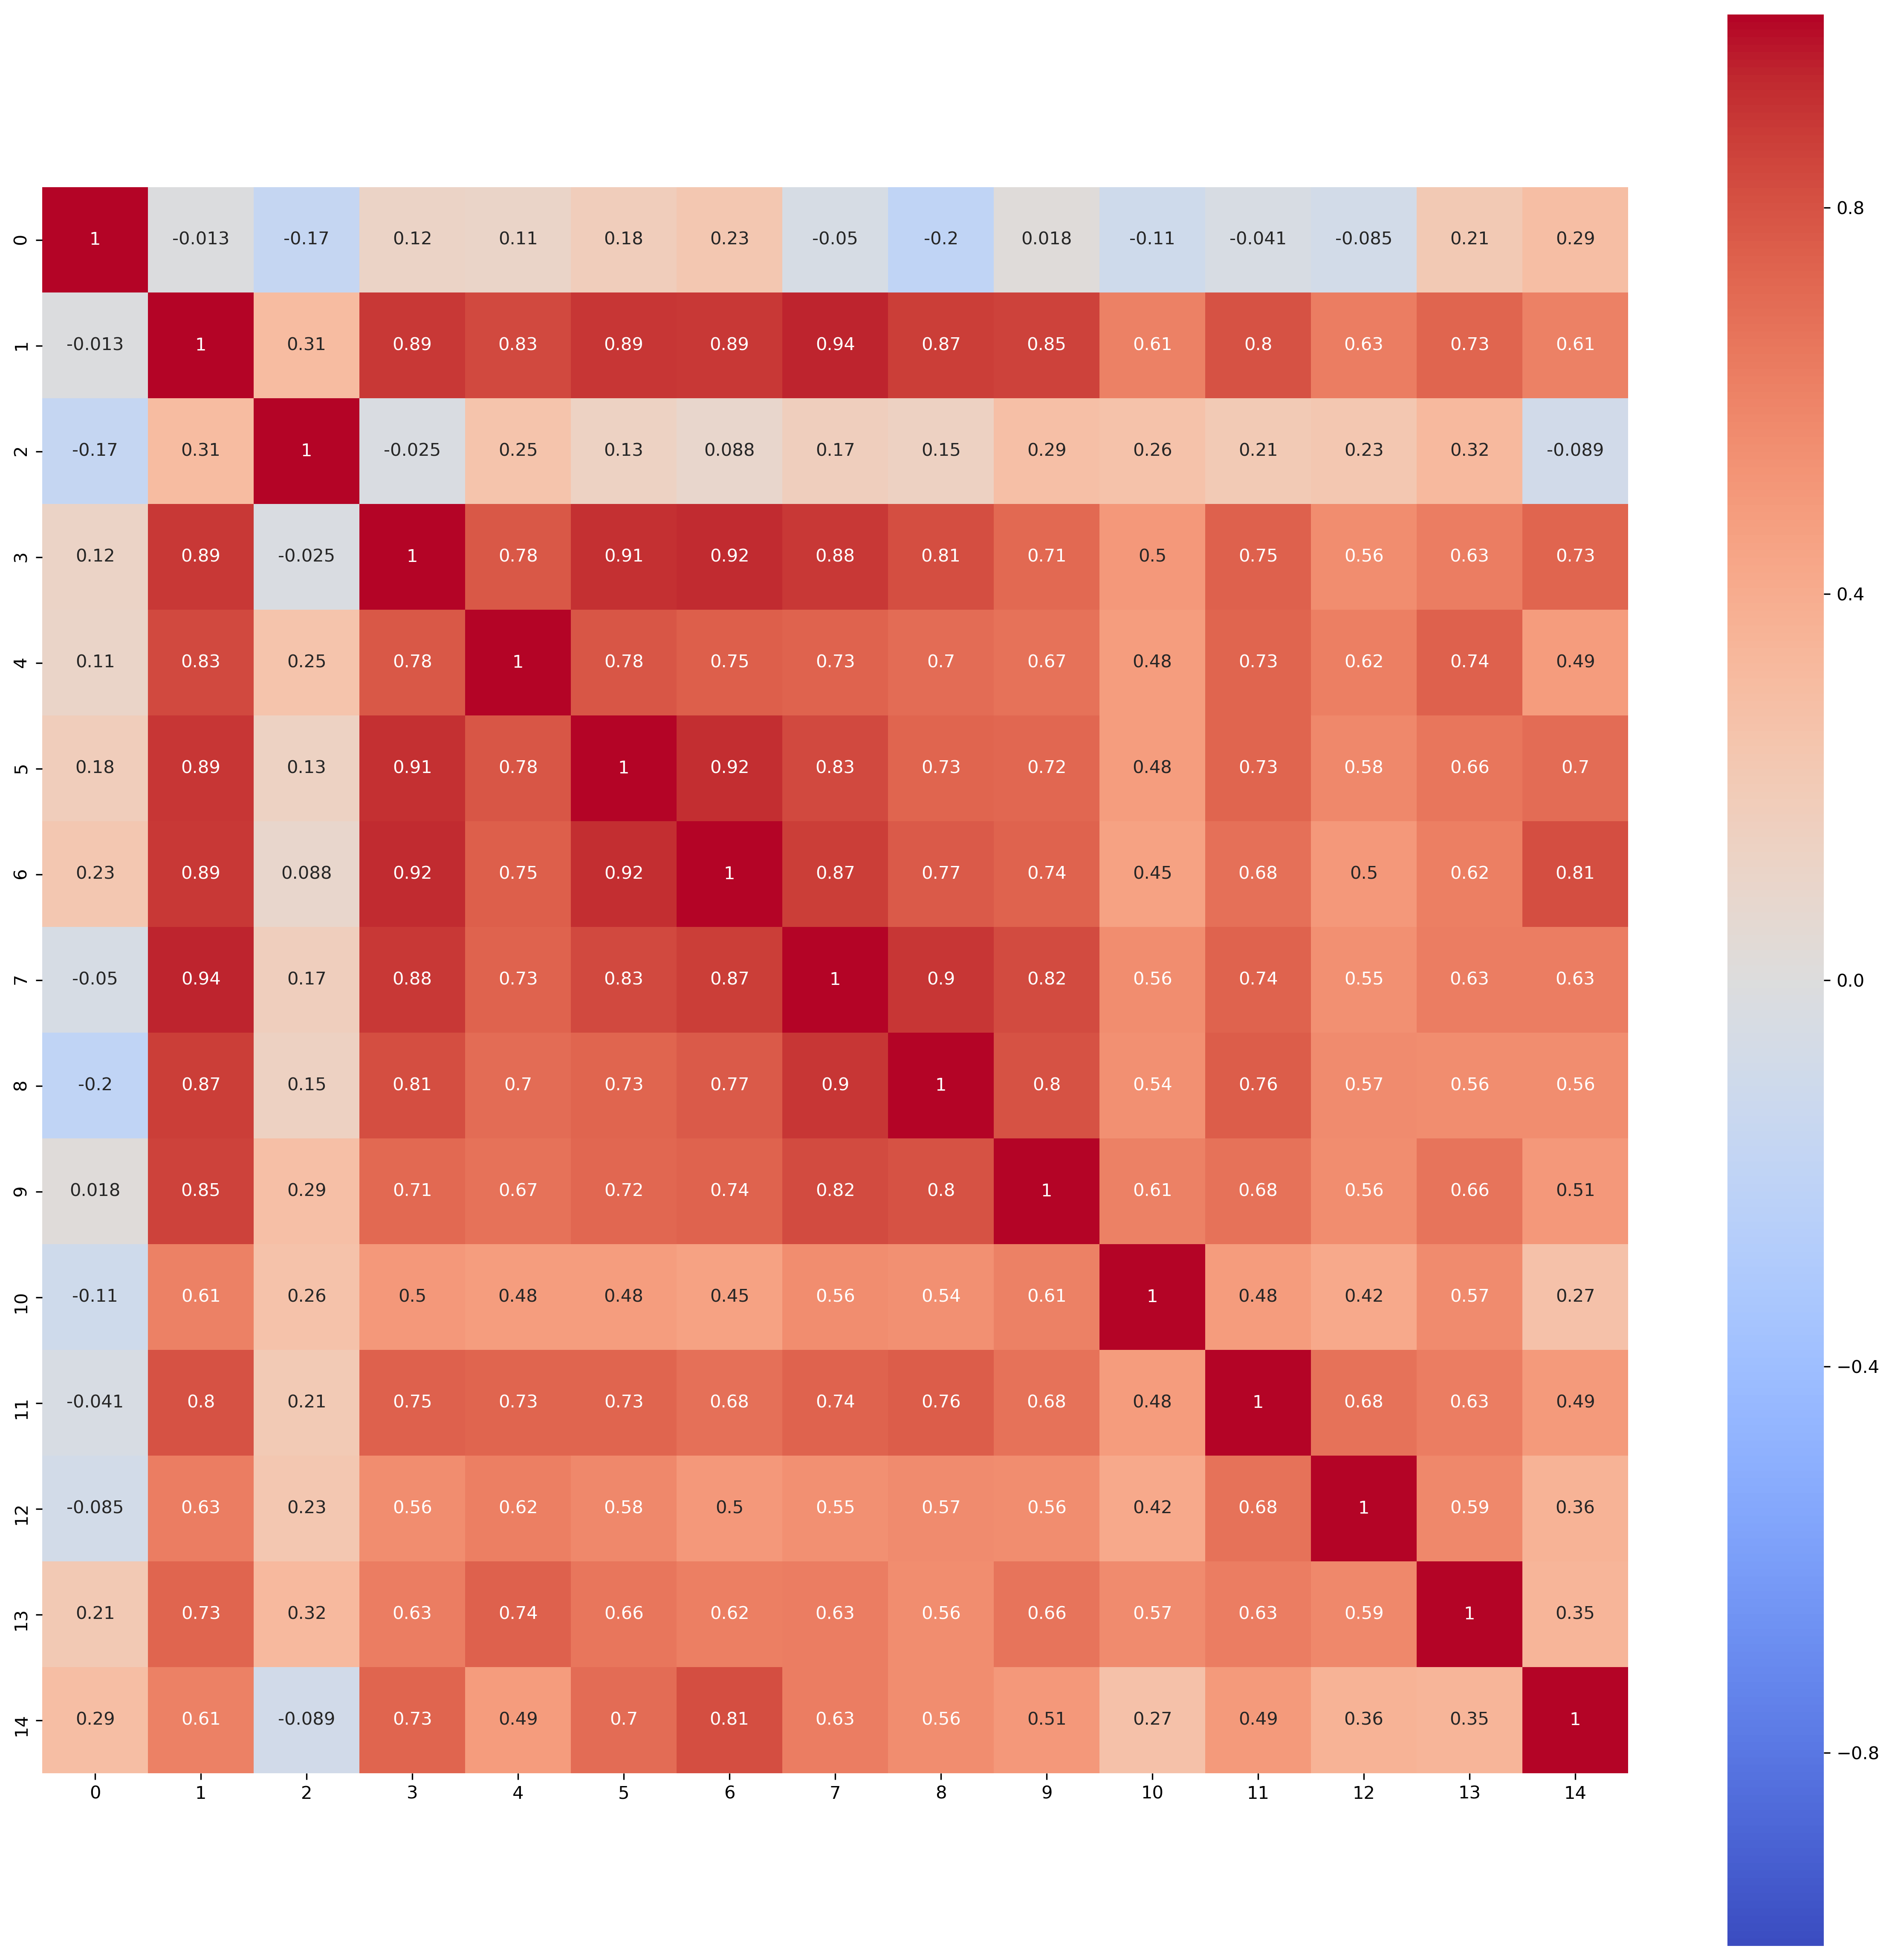
\includegraphics[width=0.5\textwidth]{correlation_heatmap}
	\caption{Correlations between recorded parameters in the data\label{fig:heatmap}}
\end{center}
\end{figure}
\end{centering}

The covariance was also computed between each parameter in the data set. Because the covariance is not normalized, it is harder to use as a tool. This is demonstrated in figure \ref{fig:cov_heatmap}, where most values fall into the \numrange{0}{50} (as shown in figure \ref{fig:cov_hist}). Covariance is not normalized, and the varying scale makes it difficult to use intuitively to identify relationships between data.

\begin{centering}
\begin{figure}
\centering
\begin{center}
	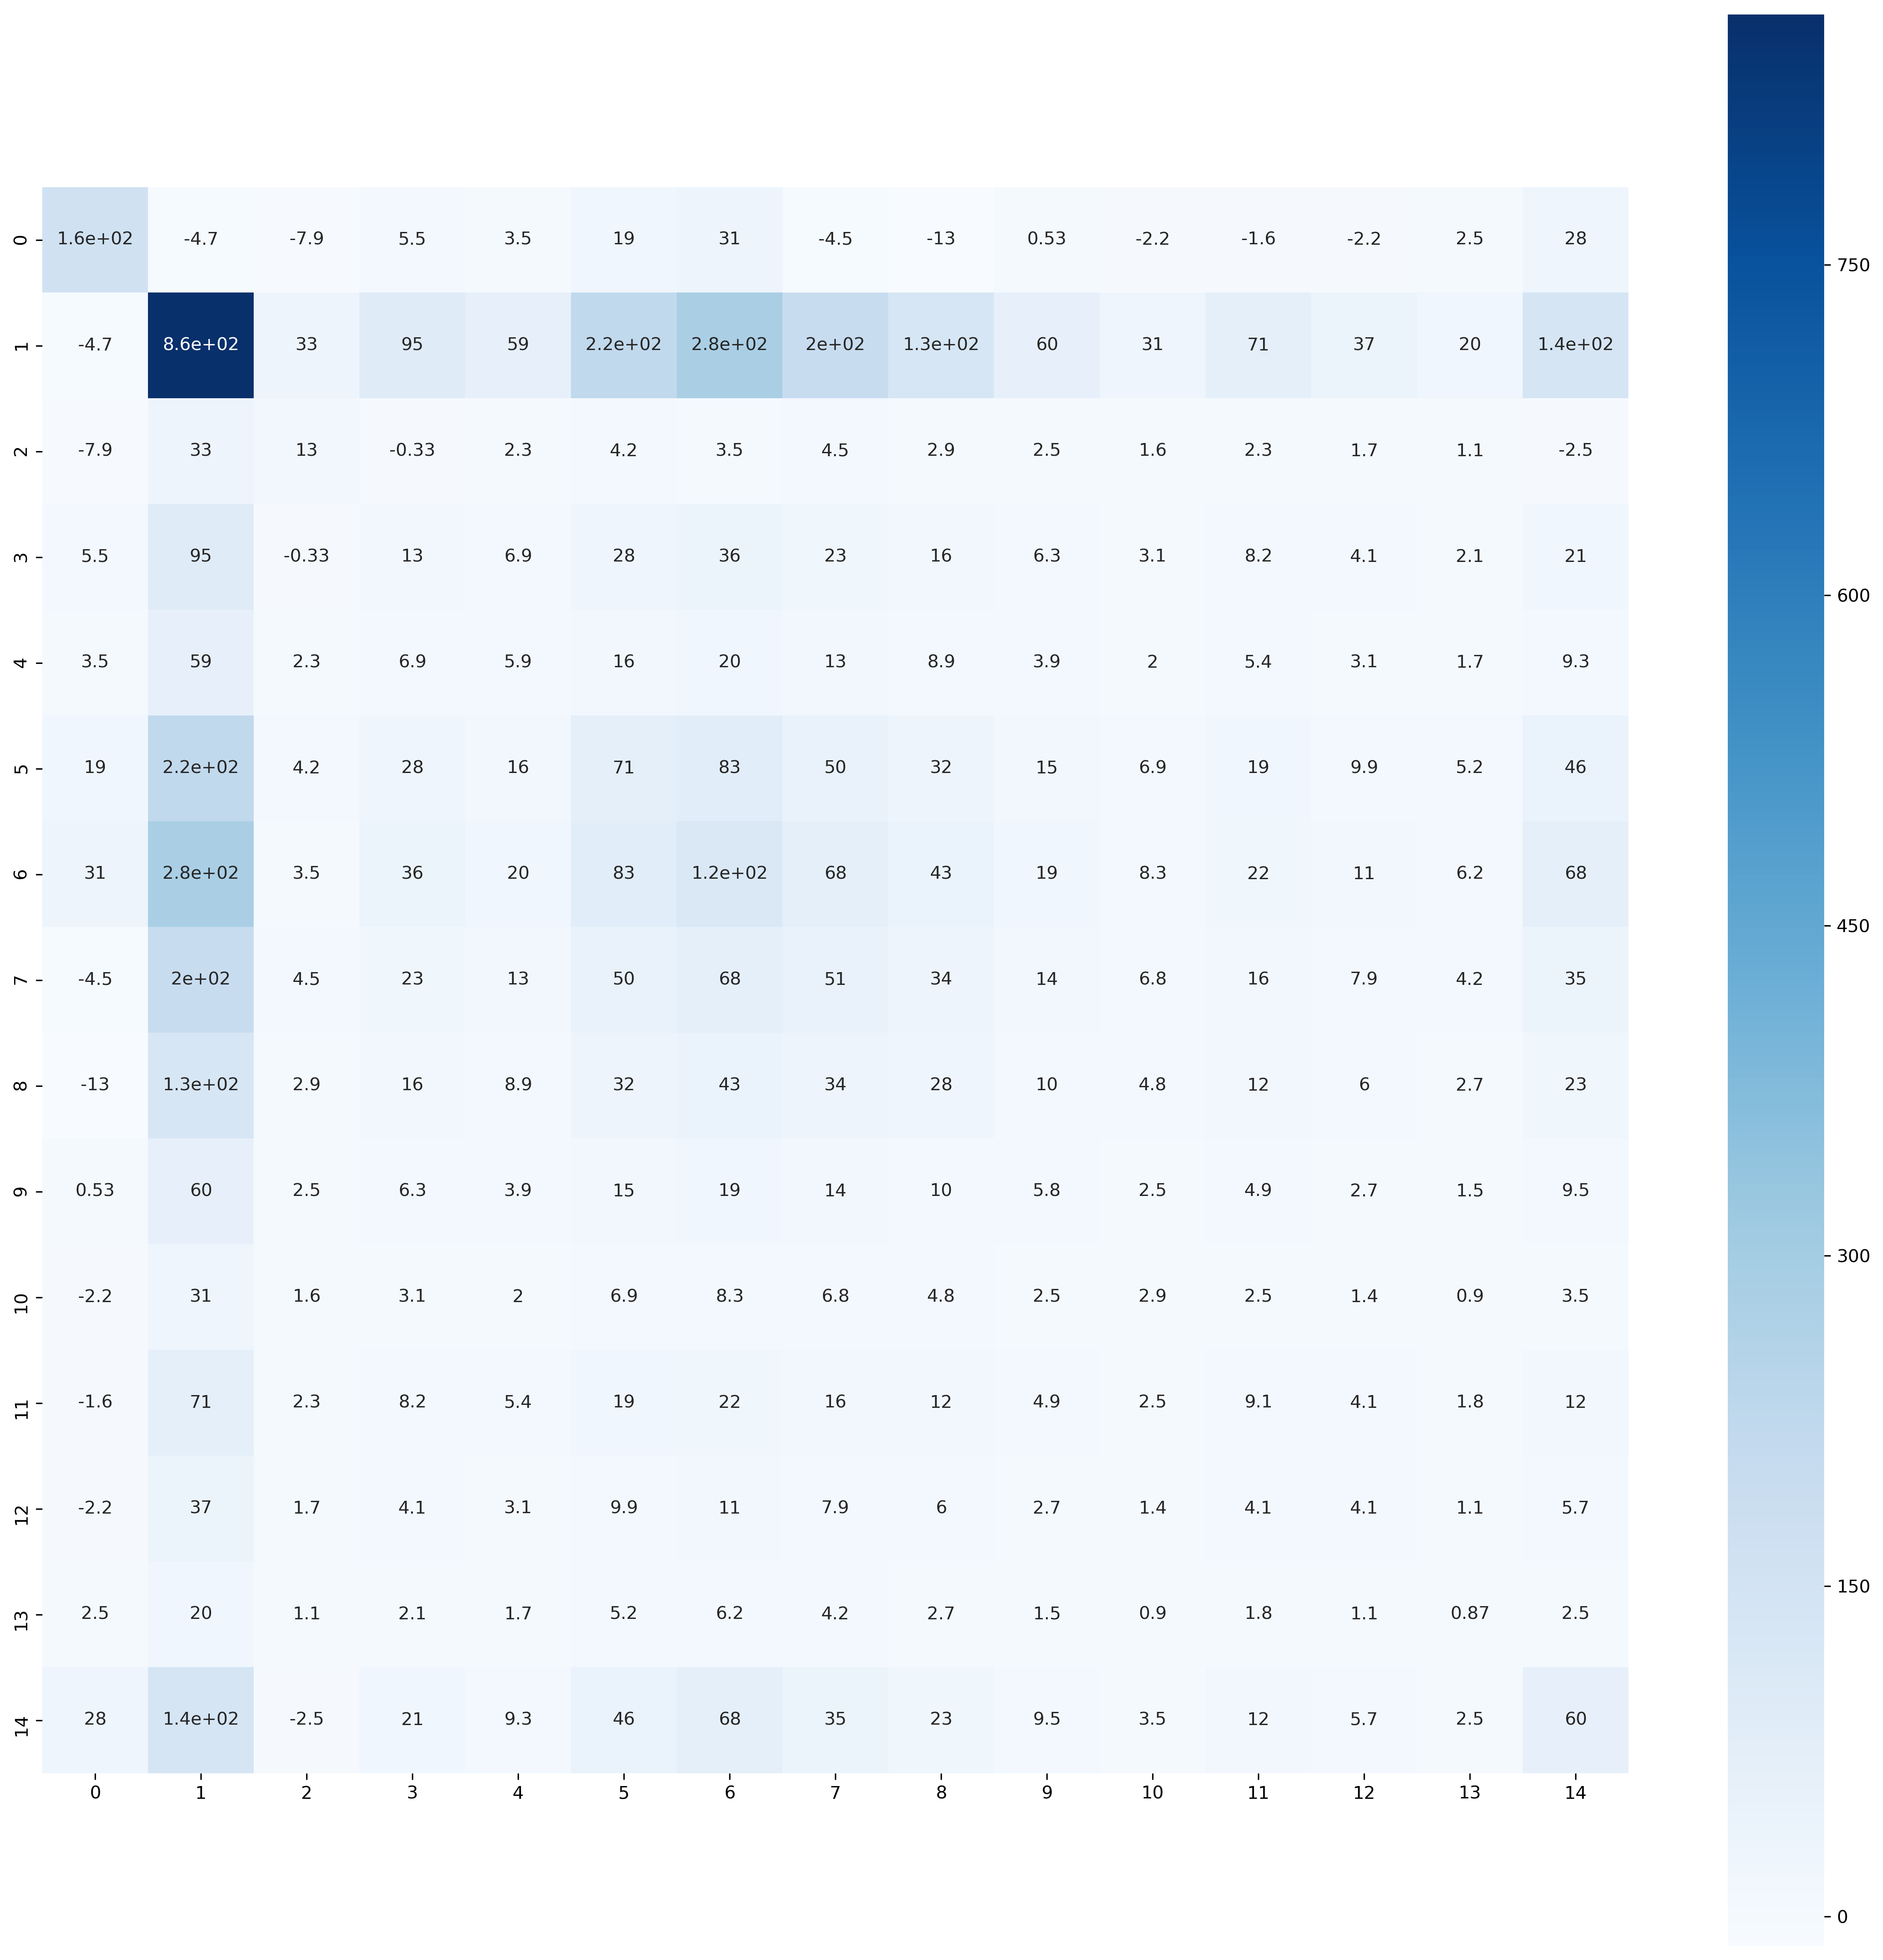
\includegraphics[width=0.5\textwidth]{covariance_heatmap}
	\caption{Correlations between recorded parameters in the data\label{fig:cov_heatmap}}
\end{center}
\end{figure}
\end{centering}

\begin{centering}
\begin{figure}
\centering
\begin{center}
	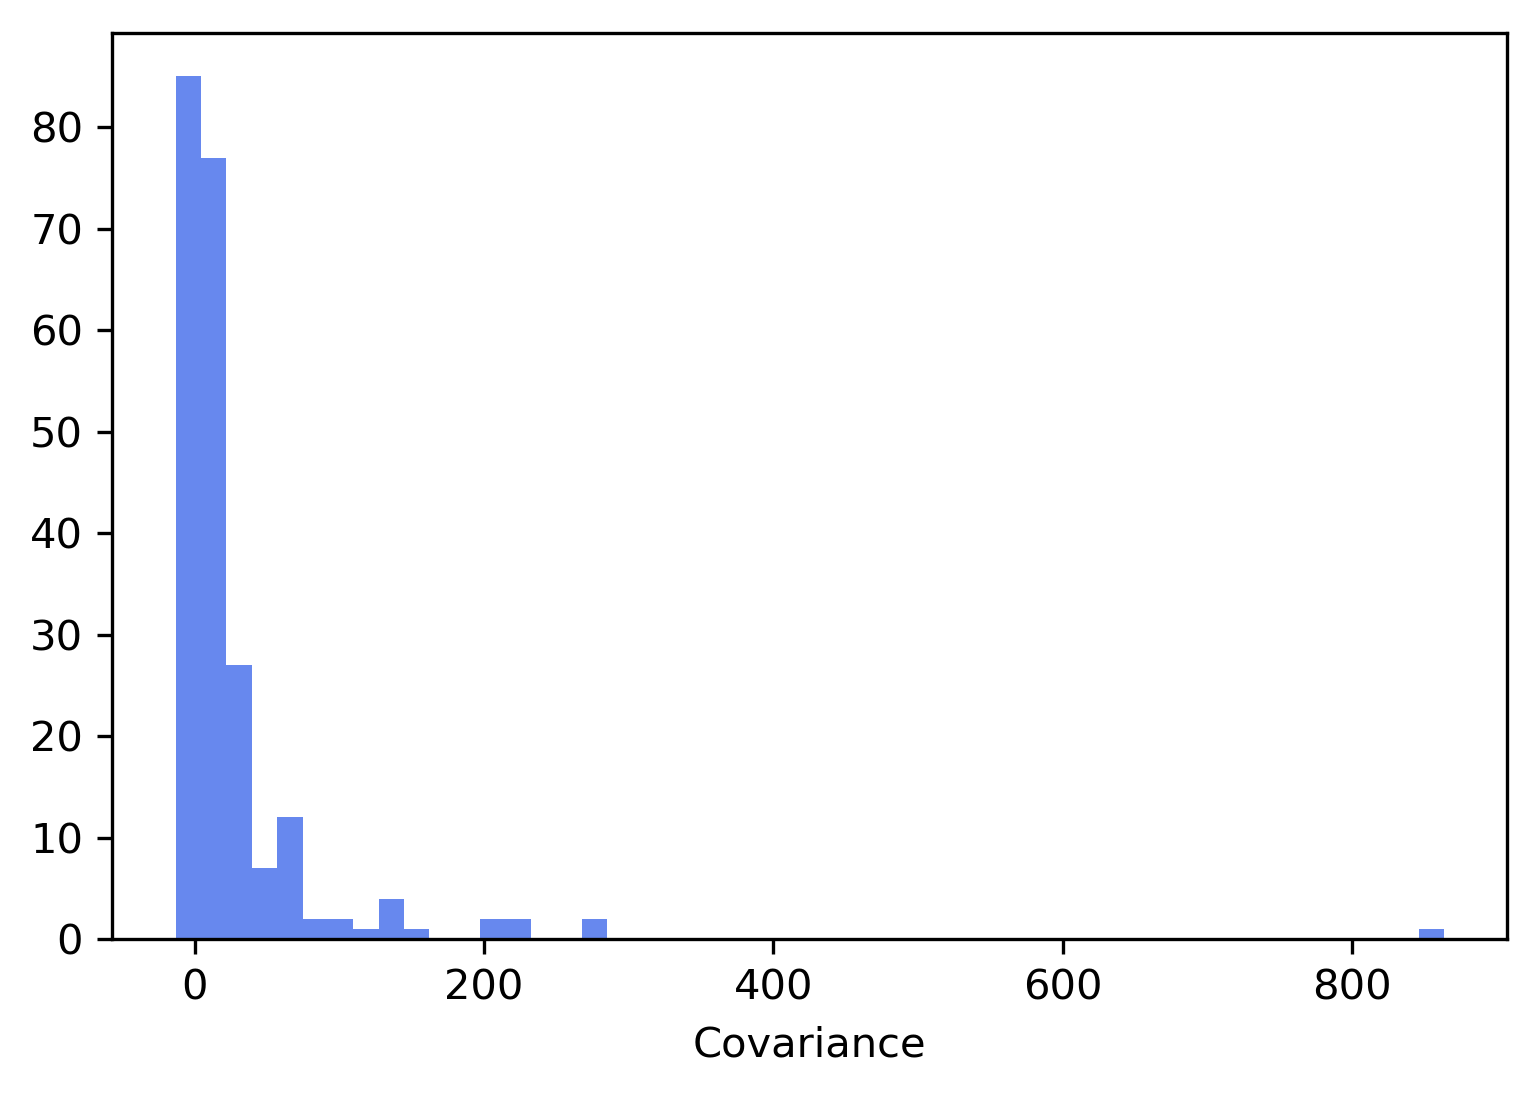
\includegraphics[width=0.5\textwidth]{covariance_dist}
	\caption{The covariance values were strongly clustered around zero, with one value (auto-covariance of weight with itself) dominating by nearly three orders of magnitude.\label{fig:cov_hist}}
\end{center}
\end{figure}
\end{centering}

\section{Conclusions}
Summary statistics calculated for a real-world data set revealed that assumptions about sampled data (e.g. that it closely follows a Gaussian or uniform distribution) may not be valid--even with a significant sample size. Statistical moments as well as other properties of a distribution such as median and trimmed mean provide a straightforward tool to approximately determine whether or not a sample conforms to a standard distribution.

These analyses reveal that the data collected deviated from the normal distribution. Further, it showed the value of carful analysis of the parameters of the sampled data, including recognizing the thresholds required to confirm or reject distribution hypotheses and the sometimes subtle nature of outliers in the data.

Values closely correlated with body fat percentage (and therefore inversely correlated with lean body mass) were identified, and the correlation of those values with other measured quantities was calculated and discussed. The correlation between circumference measurements of the torso, neck, and thighs were found to be linked (correlation \textgreater\num{0.7}), though a causal relationship could not be inferred. 

Now that the measured data are better understood, further work can be performed to see if the lean body mass formula described in equation \ref{eq:brozek} can be improved upon, possibly with a ridge regression or some other hypothesis class.

%\nocite{*}
\printbibliography

\onecolumn
\section{Appendix}
Python code used to perform calculations and generate graphics.
\lstset{frame=single}
\lstinputlisting[language=python]{appendix/appendix.py}

\end{document}